\documentclass[11pt,a4paper]{article}
\usepackage[T1]{fontenc}
\usepackage[utf8]{inputenc}
\usepackage{lmodern,microtype}
\renewcommand{\familydefault}{\sfdefault}
\usepackage[margin=19mm,headheight=14pt,headsep=10pt,footskip=25pt]{geometry}
\usepackage{xcolor,tikz,tabularx,booktabs,enumitem,titlesec,fancyhdr,lastpage}
\definecolor{ink}{HTML}{243747}
\definecolor{accent}{HTML}{126B80}
\definecolor{muted}{HTML}{506372}
\definecolor{pale}{HTML}{EFF5F7}
\definecolor{rulecolor}{HTML}{CDDCE2}
\usepackage[colorlinks=true,urlcolor=accent,linkcolor=accent,pdfauthor={Blas Manuel Rodríguez Lara},pdftitle={Inkscape Optical Elements - User Guide},pdfsubject={Version 0.6.0: free-space optical schematics},pdfkeywords={Inkscape, optics, schematic, user guide}]{hyperref}
\hypersetup{pdfcreator={pdfLaTeX},pdfdisplaydoctitle=true}
\color{ink}
\setlength{\parindent}{0pt}
\setlength{\parskip}{7pt}
\setlength{\emergencystretch}{2em}
\setlist{leftmargin=1.4em,itemsep=5pt,topsep=3pt,parsep=0pt}
\renewcommand{\arraystretch}{1.3}
\newcolumntype{Y}{>{\raggedright\arraybackslash}X}
\titleformat{\section}{\Large\bfseries\color{ink}}{}{0pt}{}
\titleformat{\subsection}{\normalsize\bfseries\color{accent}}{}{0pt}{}
\titlespacing*{\section}{0pt}{0pt}{11pt}
\titlespacing*{\subsection}{0pt}{10pt}{3pt}
\pagestyle{fancy}
\fancyhf{}
\fancyhead[L]{\small\color{muted}INKSCAPE OPTICAL ELEMENTS}
\fancyhead[R]{\small\color{muted}USER GUIDE / 0.6.0}
\fancyfoot[L]{\small\color{muted}Free-space optical schematics}
\fancyfoot[R]{\small\color{muted}\thepage\ / \pageref*{LastPage}}
\renewcommand{\headrulewidth}{0.4pt}
\renewcommand{\footrulewidth}{0pt}
\newcommand{\guidepage}[2]{\clearpage\pdfbookmark[0]{#1 - #2}{guide-#1}\section*{\textcolor{accent}{#1}\quad #2}}
\newcommand{\note}[2]{\par\smallskip\noindent\colorbox{pale}{\parbox{\dimexpr\linewidth-18pt\relax}{\vspace{5pt}\textbf{#1}\par\vspace{3pt}#2\vspace{5pt}}}\par\smallskip}
\newcommand{\menu}{\textbf{Extensions $\rightarrow$ Optical Elements $\rightarrow$ Build System\ldots}}
\newcommand{\filepath}[1]{\texttt{\detokenize{#1}}}
\begin{document}
\pdfbookmark[0]{01 - Install and start}{guide-01}

{\color{accent}\small VERSION 0.6.0\quad /\quad EXPERIMENTAL PRE-RELEASE}\par
{\fontsize{27}{31}\selectfont\bfseries Inkscape Optical Elements\par}
{\Large User guide\par}
\vspace{2pt}
Drag symbols onto a grid, join their ports, and return an editable vector diagram to Inkscape. The library contains \textbf{63 free-space optical symbols} and \textbf{11 editable layouts} for linear and nonlinear optics, cavities, and interferometers.

\section*{01\quad Install and start}
\begin{enumerate}
\item Download and extract the repository ZIP. Locate the folder named \filepath{optical_elements_builder}.
\item In Inkscape, open \textbf{Preferences $\rightarrow$ System}. Find the directory labeled \textbf{User extensions}. The Preferences menu location varies by operating system.
\item Copy the entire \filepath{optical_elements_builder} folder into that directory. Keep all its files and its \filepath{optical_builder} subfolder together.
\item Restart Inkscape. Open or create a document, then choose \menu.
\end{enumerate}

\note{One folder to copy}{Only \filepath{optical_elements_builder} belongs in the User extensions directory. The documentation and examples can stay elsewhere. There is no installer to run and no separate application to launch.}

\subsection*{Runtime and compatibility}
Inkscape's selected Python interpreter must provide \textbf{Python 3.9 or later and Tkinter}. Copying the folder does not install these requirements. Development and regression checks used \textbf{macOS, Inkscape 1.4.4, Python 3.14.7, and Tk 8.6}. Other versions and Windows/Linux have not been validated for this release.

The extension opens a separate editor window through Inkscape. Inkscape waits until you choose \textbf{Apply to Inkscape} or \textbf{Cancel}. The editor is not an Inkscape dock. If no window appears, use the troubleshooting table on page~\pageref{troubleshooting}.

\subsection*{Where to go next}
\begin{tabularx}{\linewidth}{@{}lY@{}}
\toprule
Page & Task \\
\midrule
2 & Build and reopen the simple mirror example. \\
3-4 & Select, connect, rotate, and align components. \\
5-6 & Explore the library, save drawings, and resolve common errors. \\
7-8 & Read the scope, caveat emptor notice, license, and references. \\
\bottomrule
\end{tabularx}

\guidepage{02}{A simple mirror system}
Open \filepath{examples/simple_mirror_system.svg} in Inkscape, select the optical system, and choose \textbf{Build System\ldots} to inspect the finished example. To make it yourself, start with a blank document and follow the steps below.

\begin{center}
\begin{tikzpicture}[x=0.023cm,y=-0.023cm,line cap=round,line join=round]
\path[use as bounding box] (60,100) rectangle (490,355);
\draw[ink,line width=0.85pt] (160.00000,280.00000) -- (420.00000,280.00000);
\draw[ink,line width=0.85pt] (420.00000,280.00000) -- (280.00000,160.00000);
\draw[ink,line width=1pt] (80.00000,260.00000) -- (140.00000,260.00000) -- (140.00000,300.00000) -- (80.00000,300.00000) -- (80.00000,260.00000) -- (80.00000,260.00000);
\draw[ink,line width=1pt] (140.00000,280.00000) -- (160.00000,280.00000);
\draw[ink,line width=1pt] (88.00000,280.00000) -- (132.00000,280.00000);
\filldraw[draw=accent,fill=white,line width=0.8pt] (160.0000,280.0000) circle[radius=2.7];
\node[font=\small,text=ink] at (120,335) {Laser};
\draw[ink,line width=1pt] (424.49900,239.01514) -- (424.76736,241.77998) -- (424.96245,244.51772) -- (425.08425,247.22835) -- (425.13278,249.91188) -- (425.10805,252.56830) -- (425.01005,255.19762) -- (424.83877,257.79983) -- (424.59421,260.37493) -- (424.27639,262.92294) -- (423.88530,265.44384) -- (423.42093,267.93762) -- (422.88328,270.40431) -- (422.27237,272.84389) -- (421.58820,275.25637) -- (420.83073,277.64174) -- (420.00000,280.00000) -- (419.09600,282.33116) -- (418.11873,284.63522) -- (417.06818,286.91217) -- (415.94436,289.16201) -- (414.74727,291.38475) -- (413.47691,293.58039) -- (412.13327,295.74891) -- (410.71636,297.89033) -- (409.22618,300.00465) -- (407.66274,302.09187) -- (406.02601,304.15198) -- (404.31601,306.18498) -- (402.53274,308.19088) -- (400.67621,310.16967) -- (398.74639,312.12136) -- (396.74330,314.04594);
\draw[ink,line width=1pt] (428.25054,240.40292) -- (428.51890,243.16777) -- (428.71399,245.90551) -- (428.83579,248.61614) -- (428.88432,251.29966) -- (428.85959,253.95608) -- (428.76157,256.58540) -- (428.59031,259.18761) -- (428.34575,261.76272) -- (428.02793,264.31072) -- (427.63684,266.83162) -- (427.17247,269.32541) -- (426.63482,271.79209) -- (426.02391,274.23167) -- (425.33972,276.64415) -- (424.58227,279.02952) -- (423.75154,281.38778) -- (422.84754,283.71895) -- (421.87025,286.02300) -- (420.81972,288.29995) -- (419.69590,290.54979) -- (418.49881,292.77253) -- (417.22845,294.96817) -- (415.88481,297.13670) -- (414.46790,299.27812) -- (412.97773,301.39244) -- (411.41426,303.47965) -- (409.77755,305.53976) -- (408.06755,307.57276) -- (406.28428,309.57866) -- (404.42775,311.55746) -- (402.49793,313.50914) -- (400.49484,315.43372);
\filldraw[draw=accent,fill=white,line width=0.8pt] (420.0000,280.0000) circle[radius=2.7];
\node[font=\small,text=ink] at (420,335) {M1 (CM)};
\draw[ink,line width=1pt] (253.96835,190.37026) -- (306.03165,129.62974);
\draw[ink,line width=1pt] (250.93132,187.76710) -- (302.99463,127.02657);
\draw[ink,line width=1pt] (256.13765,181.69305) -- (255.26993,170.41266);
\draw[ink,line width=1pt] (269.15348,166.50791) -- (268.28576,155.22753);
\draw[ink,line width=1pt] (282.16930,151.32278) -- (281.30158,140.04240);
\draw[ink,line width=1pt] (295.18513,136.13765) -- (294.31741,124.85727);
\filldraw[draw=accent,fill=white,line width=0.8pt] (280.0000,160.0000) circle[radius=2.7];
\node[font=\small,text=ink] at (280,215) {M2};
\end{tikzpicture}

\end{center}
{\small\color{muted}Example geometry from the extension. Blue circles show connection ports in the builder; they do not appear in the exported drawing. M1 is a concave folding mirror. M2 is a plane end mirror.}

\begin{enumerate}
\item \textbf{Place three symbols.} Search the gallery for \textbf{Laser}, \textbf{Concave mirror}, and \textbf{Plane mirror}. Drag each onto the grid. Place the laser at the left, the concave mirror to its right at the same height, and the plane mirror above and to the left of the concave mirror. Use the arrangement above as a guide.
\item \textbf{Name the mirrors.} Select a component, enter its label in \textbf{Label}, and press Return. The example uses \textbf{Laser}, \textbf{M1 (CM)}, and \textbf{M2}.
\item \textbf{Join the first path.} Set \textbf{Connections} to \textbf{Straight}. Drag from the laser's blue output port to the central port of M1. Release over the target circle.
\item \textbf{Join the second path.} Drag from M1's same central port to the central port of M2. M1 rotates to reflect between the two directions. M2 turns to face M1 at normal incidence. Both segments remain attached to their ports.
\item \textbf{Try moving a mirror.} Drag the body of M2 to another grid position. The paths and mirror orientations update. If you previously entered manual angles, clear the selection and click \textbf{Align optics} to restore automatic alignment throughout the system.
\item \textbf{Apply and return.} Click \textbf{Apply to Inkscape}, then save an SVG. Select the system in Inkscape and reopen \textbf{Build System\ldots} to continue editing. Save a new copy if you want to retain the supplied example.
\end{enumerate}

\note{What this example shows}{It demonstrates placement, attached paths, reflection alignment, and reopening. M2 has only one connected direction, so its return path overlaps the incoming path and is not drawn separately. No focal length, beam waist, or physical spacing is specified.}

\guidepage{03}{Edit components and connections}
Use the category selector or search box to find a component. Dragging a thumbnail places a new instance. Component centers snap to a fixed \textbf{20-pixel grid in builder coordinates}; this is a drawing grid, not a physical length scale.

\begin{tabularx}{\linewidth}{@{}>{\raggedright\arraybackslash}p{0.26\linewidth}Y@{}}
\toprule
\textbf{Action} & \textbf{Control} \\
\midrule
Select one & Click the component body. Clicking near a port starts a connection instead. \\
Select several & Shift-click to add or remove components. Drag a rectangle from blank canvas to select components whose centers lie inside it. Shift-drag adds to the selection. \\
Select everything & Click \textbf{Select all}, or use Cmd+A on Mac / Ctrl+A elsewhere while the canvas has focus. \\
Move a selection & Drag a selected component body. Every selected component receives the same snapped displacement. Spacing is preserved; attached paths update. \\
Clear a selection & Click blank canvas. \\
Connect ports & Drag from one blue port to another. Select \textbf{Straight} or \textbf{Right angles} before drawing a new connection. \\
Remove a connection & Click the line away from components, then click \textbf{Delete}. To change an existing route, delete and redraw it with the desired routing mode. \\
Delete components & Select them and click \textbf{Delete}, or press Delete/Backspace with canvas focus. Their attached connections are removed too. \\
Undo / redo & Use the toolbar buttons. With canvas focus, Cmd/Ctrl+Z undoes; Shift+Cmd/Ctrl+Z redoes. Selection moves and inserted layouts are single undo operations. \\
Cancel a drag & Press Escape before releasing the mouse. A cancelled move restores the starting positions. \\
Change a label & Select one component, edit \textbf{Label}, and press Return. Labels describe the intended device or function. \\
View the canvas & Use the $-$ and $+$ zoom buttons and the scrollbars. The mouse wheel scrolls vertically. \\
\bottomrule
\end{tabularx}

\subsection*{Rotate by any angle}
Select one component. Enter a finite positive, negative, or decimal value in \textbf{Angle $^\circ$}, then press Return or \textbf{Set angle}. Positive values rotate clockwise from the symbol's original orientation. Press \textbf{R} with canvas focus to jump to the angle field.

Setting a manual angle switches off \textbf{Follow beams} for that component. Check \textbf{Follow beams} again to restore automatic alignment where the component supports it. An angle is a symbol rotation, not a polarization or incidence-angle setting.

\note{Connecting after moving a group}{While several components are selected, dragging a port on a selected component moves the group. Click blank canvas first, then drag the individual ports you want to join. This also applies just after inserting a layout.}

\guidepage{04}{How alignment works}
Eligible components follow the connected beam directions as you connect or move them. Alignment changes their rotations and leaves their centers in place.

\begin{center}
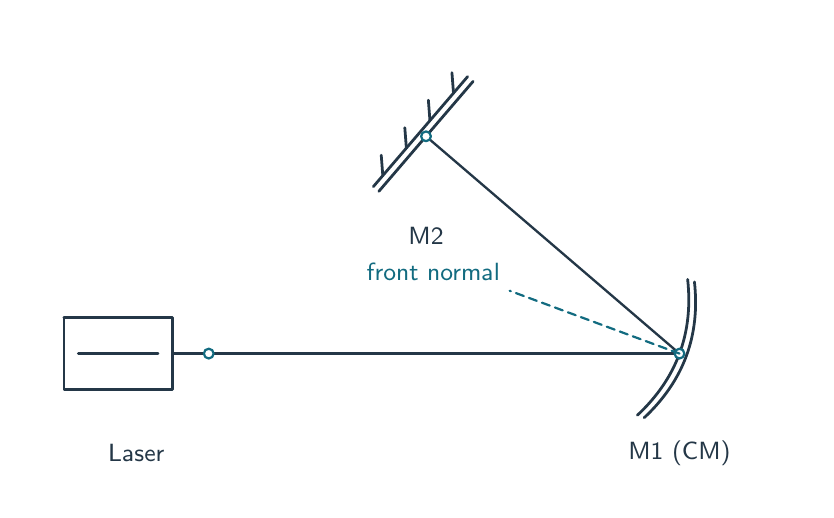
\begin{tikzpicture}[x=0.023cm,y=-0.023cm,line cap=round,line join=round]
\path[use as bounding box] (60,100) rectangle (490,355);
\draw[ink,line width=0.85pt] (160.00000,280.00000) -- (420.00000,280.00000);
\draw[ink,line width=0.85pt] (420.00000,280.00000) -- (280.00000,160.00000);
\draw[ink,line width=1pt] (80.00000,260.00000) -- (140.00000,260.00000) -- (140.00000,300.00000) -- (80.00000,300.00000) -- (80.00000,260.00000) -- (80.00000,260.00000);
\draw[ink,line width=1pt] (140.00000,280.00000) -- (160.00000,280.00000);
\draw[ink,line width=1pt] (88.00000,280.00000) -- (132.00000,280.00000);
\filldraw[draw=accent,fill=white,line width=0.8pt] (160.0000,280.0000) circle[radius=2.7];
\node[font=\small,text=ink] at (120,335) {Laser};
\draw[ink,line width=1pt] (424.49900,239.01514) -- (424.76736,241.77998) -- (424.96245,244.51772) -- (425.08425,247.22835) -- (425.13278,249.91188) -- (425.10805,252.56830) -- (425.01005,255.19762) -- (424.83877,257.79983) -- (424.59421,260.37493) -- (424.27639,262.92294) -- (423.88530,265.44384) -- (423.42093,267.93762) -- (422.88328,270.40431) -- (422.27237,272.84389) -- (421.58820,275.25637) -- (420.83073,277.64174) -- (420.00000,280.00000) -- (419.09600,282.33116) -- (418.11873,284.63522) -- (417.06818,286.91217) -- (415.94436,289.16201) -- (414.74727,291.38475) -- (413.47691,293.58039) -- (412.13327,295.74891) -- (410.71636,297.89033) -- (409.22618,300.00465) -- (407.66274,302.09187) -- (406.02601,304.15198) -- (404.31601,306.18498) -- (402.53274,308.19088) -- (400.67621,310.16967) -- (398.74639,312.12136) -- (396.74330,314.04594);
\draw[ink,line width=1pt] (428.25054,240.40292) -- (428.51890,243.16777) -- (428.71399,245.90551) -- (428.83579,248.61614) -- (428.88432,251.29966) -- (428.85959,253.95608) -- (428.76157,256.58540) -- (428.59031,259.18761) -- (428.34575,261.76272) -- (428.02793,264.31072) -- (427.63684,266.83162) -- (427.17247,269.32541) -- (426.63482,271.79209) -- (426.02391,274.23167) -- (425.33972,276.64415) -- (424.58227,279.02952) -- (423.75154,281.38778) -- (422.84754,283.71895) -- (421.87025,286.02300) -- (420.81972,288.29995) -- (419.69590,290.54979) -- (418.49881,292.77253) -- (417.22845,294.96817) -- (415.88481,297.13670) -- (414.46790,299.27812) -- (412.97773,301.39244) -- (411.41426,303.47965) -- (409.77755,305.53976) -- (408.06755,307.57276) -- (406.28428,309.57866) -- (404.42775,311.55746) -- (402.49793,313.50914) -- (400.49484,315.43372);
\filldraw[draw=accent,fill=white,line width=0.8pt] (420.0000,280.0000) circle[radius=2.7];
\node[font=\small,text=ink] at (420,335) {M1 (CM)};
\draw[ink,line width=1pt] (253.96835,190.37026) -- (306.03165,129.62974);
\draw[ink,line width=1pt] (250.93132,187.76710) -- (302.99463,127.02657);
\draw[ink,line width=1pt] (256.13765,181.69305) -- (255.26993,170.41266);
\draw[ink,line width=1pt] (269.15348,166.50791) -- (268.28576,155.22753);
\draw[ink,line width=1pt] (282.16930,151.32278) -- (281.30158,140.04240);
\draw[ink,line width=1pt] (295.18513,136.13765) -- (294.31741,124.85727);
\filldraw[draw=accent,fill=white,line width=0.8pt] (280.0000,160.0000) circle[radius=2.7];
\node[font=\small,text=ink] at (280,215) {M2};
\draw[accent,densely dashed,line width=0.8pt] (420,280) -- (326.21150,245.30538);
\node[font=\small,text=accent,anchor=south east] at (326.21150,245.30538) {front normal};
\end{tikzpicture}

\end{center}
{\small\color{muted}The dashed line is the outward surface normal at M1's vertex. It bisects the two directions pointing away from the mirror toward its connected neighbors. The coating faces both paths. The dashed normal is a guide annotation.}

\subsection*{Mirrors}
With \textbf{two distinct connected directions}, the mirror follows the local law of reflection. With \textbf{one direction}, it acts as an end mirror at normal incidence. Plane, concave, convex, and the other supported mirror variants use the same rule at their central port. Curved symbols use the normal at the vertex; no focusing calculation is performed.

\subsection*{Other optics}
Sources, detectors, straight-through optics, and supported beam-splitter axes rotate when the connected directions match the symbol's fixed port geometry. An impossible arrangement, such as a straight-through lens joining noncollinear paths, cannot be corrected by rotation alone.

Prisms, diffraction gratings, Wollaston prisms, noncollinear nonlinear crystals, AOM deflection, and screens remain manual. Their behavior requires device-specific information or a choice of display orientation. The \textbf{Follow beams} control is disabled for unsupported symbols.

\subsection*{Restore alignment or handle a warning}
Click \textbf{Align optics} to restore automatic alignment for the selected components. With no components selected, it restores automatic alignment throughout the system. Other components already following beams may also adjust as connected directions change.

An \textbf{amber outline} marks an ambiguous or incompatible arrangement. The status line explains the issue. Move a component, use a compatible port, or remove an unintended connection. For example, more than two distinct directions at a mirror do not define one reflection angle. The editor still allows Apply, so inspect warnings before exporting.

\note{Connections remain schematic}{For a right-angle route, alignment uses the segment that touches the element. An elbow in a line does not insert a physical mirror. A missing warning does not establish physical validity, and manually fixed angles are not checked by the automatic solver.}

\guidepage{05}{Symbols and editable layouts}
The gallery contains free-space optics only. Symbols use common laboratory drawing conventions and identifying labels. This is not an ISO-certified symbol set; supply the labels and legend your audience needs.

\begin{tabularx}{\linewidth}{@{}Yr>{\raggedright\arraybackslash}p{0.43\linewidth}@{}}
\toprule
\textbf{Family} & \textbf{Count} & \textbf{Typical contents} \\
\midrule
Sources and detection & 7 & Lasers, detectors, cameras, screens \\
Mirrors and beam splitters & 11 & Plane/curved mirrors, beam splitters, plate splitters, dichroics \\
Lenses and focusing & 9 & Converging/diverging, cylindrical, and other lens forms \\
Polarization & 10 & Polarizers, wave plates, PBS, rotators, isolator \\
Apertures and filters & 9 & Stops, apertures, spatial and spectral filters \\
Prisms and diffraction & 6 & Prisms, gratings, diffraction elements \\
Nonlinear and active media & 11 & Crystals, gain, absorbers, modulators, cells \\
\bottomrule
\end{tabularx}

\subsection*{Eleven ready-made layouts}
Select \textbf{Cavities and layouts}, then drag a thumbnail onto the grid. Each layout inserts ordinary editable components and connections, selected together. Move the assembly immediately, or click blank canvas and edit individual components.

\begin{tabularx}{\linewidth}{@{}>{\raggedright\arraybackslash}p{0.26\linewidth}Y@{}}
\toprule
\textbf{Group} & \textbf{Layouts} \\
\midrule
Cavities & Fabry-P\'erot, linear laser, four-mirror ring, bow-tie \\
Interferometers & Michelson, Mach-Zehnder, Sagnac \\
Nonlinear optics & Second-harmonic generation; noncollinear SPDC source \\
Beam preparation & Spatial filter / 4f relay; polarization preparation / analysis \\
\bottomrule
\end{tabularx}

\subsection*{Use labels to identify the actual device}
Some devices share an outline. A wave plate labeled $\lambda/2$ or $\lambda/4$, for example, communicates a different role without a different housing shape. Change labels to specify material, retardance, wavelength, or function. These labels do not configure a physical simulation.

A three-port BS or PBS displays three exposed drawing channels. It does not imply that a reciprocal physical beam splitter has only three optical modes. Ports do not enforce input/output direction or calculate splitting ratios.

\note{Complete reference and examples}{\filepath{documentation/Symbol_Reference.md} lists every symbol, initial label, port count, and layout. \filepath{examples/mach_zehnder.svg} is an additional editable example. Templates show topology; their distances, curvatures, and parameters are not optimized optical prescriptions.}

\guidepage{06}{Save, reopen, and troubleshoot}
\label{troubleshooting}
After \textbf{Apply to Inkscape}, save an \textbf{SVG master}. The file contains both visible vector paths and the builder's editable data. Select the intended optical system before reopening the extension, especially when a document contains several systems.

Moving or scaling the complete output group in Inkscape preserves its placement on reopening. Continue component, connection, label, and angle edits inside the builder. Direct edits to individual generated paths, styles, or text can block reopening; the extension stops to preserve those edits. Ungrouping or stripping metadata can also break the editable association.

\textbf{Cancel}, or closing the builder window, returns the original document. PDF and PNG exports preserve appearance but do not contain the editable builder model. Keep your SVG and a backup even when your final figure is exported to another format.

\begin{tabularx}{\linewidth}{@{}>{\raggedright\arraybackslash}p{0.31\linewidth}Y@{}}
\toprule
\textbf{Symptom} & \textbf{What to do} \\
\midrule
The menu item is missing & Check the \textbf{User extensions} path in Preferences. Copy the actual \filepath{optical_elements_builder} folder there, then restart. Do not leave it inside an extra repository or ZIP folder. \\
No window, or a Tkinter / \filepath{_tkinter} error & The Python interpreter selected by Inkscape must include Tkinter. Having it in a different Python environment is insufficient. Check that interpreter before changing extension files. \\
An old ``No module named gi'' error & This release does not import \filepath{gi}. Check for an older Optical Elements installation or duplicate files. Close Inkscape, back up the old extension, replace it with this folder, and restart. \\
``Edited outside the builder'' & Preserve the SVG. Undo the edits to generated components, or reopen a previous builder-saved copy. The extension does not silently discard external edits. \\
Several systems in one SVG & Select the intended system in Inkscape, then invoke the extension again. \\
Dragging a port moves a group & Click blank canvas to clear the multiple selection, then drag between ports. \\
A component turns back & It is following its beams. Set the angle explicitly using \textbf{Set angle}; that disables automatic alignment for this component. \\
An amber component outline & Read the status line. Check the connected ports, directions, and spacing. See page 4 for the alignment limits. \\
\bottomrule
\end{tabularx}

\subsection*{Updates, removal, and problem reports}
Close Inkscape before replacing or removing the installed extension folder. Back up the old folder and your SVGs before updating. Saved drawings remain SVG files after removal. For a report, include the OS, Inkscape version, exact error, steps to reproduce, and a minimal SVG you may share. Remove private content first.

\guidepage{07}{Caveat emptor and intended scope}
\note{Experimental software, provided as is}{This extension is a schematic drawing tool. It provides no warranty of correctness, suitability, continued maintenance, or compatibility with every Inkscape/Python installation. The full MIT license on the next page contains the permission, warranty, and liability terms.}

\subsection*{A drawing is not an optical design calculation}
Automatic alignment checks limited local geometry. It does not trace rays through a physical system or propagate optical fields. The extension does not calculate or verify:
\begin{itemize}
\item focal lengths, imaging distances, aberrations, beam waists, diffraction, or Gaussian beam evolution;
\item refraction, coating spectra, losses, polarization transformations, splitting ratios, coherence, or nonlinear phase matching;
\item cavity stability, manufacturing tolerances, laser power, damage thresholds, or apparatus safety.
\end{itemize}
Curvature in a mirror symbol does not supply a radius. Grid spacing does not specify real distances. Layouts are drawing starting points and may omit components required in a real experiment. The absence of a warning is not evidence of a valid or complete optical system.

\subsection*{Review before use}
Verify component identities, paths, labels, units, and exported figures before relying on or publishing them. Assess real apparatus independently using optical design methods, manufacturer specifications, and applicable laboratory procedures. This tool supplies no laser-safety assessment, interlock design, or certification.

Keep backups of your SVG master. External tools can change paths or remove the metadata needed to reopen a system. Check that your chosen save/export workflow retains what you need before using it for important work.

\subsection*{Local execution and validation status}
The runtime uses Python's standard library and Tkinter. It contains no network requests, telemetry, dependency installer, or automatic updater. It executes as a normal Python extension with the current user's permissions. The included source can be inspected; this is not a claim of a security audit.

Development checks covered model persistence, attached connections, multiple selection, undo, arbitrary angles, reflection geometry, templates, and Tk callbacks on the stated Mac environment. They do not establish compatibility with every platform or replace manual testing in your installation.

\subsection*{License and independent status}
Original project code, symbol data, SVG examples, and documentation use the \textbf{MIT license}. Keep its copyright and permission notice when redistributing copies or substantial portions. Academic acknowledgment is welcome, not an additional condition. Citation metadata is supplied in \filepath{CITATION.cff}.

This project is independent of Inkscape and is not endorsed by Inkscape or the authors of the reference works. Third-party software and embedded fonts retain their own licenses. \filepath{DISCLAIMER.md} and \filepath{THIRD_PARTY_NOTICES.md} accompany the release; they explain scope and attribution without adding restrictions to MIT.

\guidepage{08}{License and reference information}
\subsection*{MIT License}
{\small
Copyright (c) 2026 Blas Manuel Rodríguez Lara and contributors

Permission is hereby granted, free of charge, to any person obtaining a copy
of this software and associated documentation files (the ``Software''), to deal
in the Software without restriction, including without limitation the rights
to use, copy, modify, merge, publish, distribute, sublicense, and/or sell
copies of the Software, and to permit persons to whom the Software is
furnished to do so, subject to the following conditions:

The above copyright notice and this permission notice shall be included in all
copies or substantial portions of the Software.

THE SOFTWARE IS PROVIDED ``AS IS'', WITHOUT WARRANTY OF ANY KIND, EXPRESS OR
IMPLIED, INCLUDING BUT NOT LIMITED TO THE WARRANTIES OF MERCHANTABILITY,
FITNESS FOR A PARTICULAR PURPOSE AND NONINFRINGEMENT. IN NO EVENT SHALL THE
AUTHORS OR COPYRIGHT HOLDERS BE LIABLE FOR ANY CLAIM, DAMAGES OR OTHER
LIABILITY, WHETHER IN AN ACTION OF CONTRACT, TORT OR OTHERWISE, ARISING FROM,
OUT OF OR IN CONNECTION WITH THE SOFTWARE OR THE USE OR OTHER DEALINGS IN THE
SOFTWARE.
}

\subsection*{Dependencies and font notices}
Inkscape, Python, and Tcl/Tk are installed separately and retain their own licenses. They are not bundled with this extension. fontTools was used during development to prepare drawing polylines; it is not needed at runtime. LaTeX/TikZ was used to prepare this guide.

The PDF embeds subsets of Latin Modern fonts, copyright 2003-2021 B. Jackowski and J. M. Nowacki on behalf of TeX Users Groups, based on Computer Modern by Donald E. Knuth. These fonts retain the GUST Font License; the documentation folder contains that license and the referenced LPPL text. Standalone third-party font files are not included.

\subsection*{Sources and further reading}
\begin{enumerate}[itemsep=5pt]
\item \href{https://inkscape.gitlab.io/extensions/documentation/tutorial/my-first-effect-extension.html}{Inkscape: My first effect extension}. Official reference for effect extensions and the User extensions directory.
\item \href{https://ctan.org/pkg/pst-optexp}{Christoph Bersch: PST-opTeXp} and its \href{https://mirrors.mit.edu/CTAN/graphics/pstricks/contrib/pst-optexp/pst-optexp-quickref.pdf}{quick reference}. Reference for optical schematic conventions. Upstream uses LPPL 1.3c or later.
\item \href{https://www.rp-photonics.com/optical_resonators.html}{Rüdiger Paschotta: Optical Resonators, RP Photonics Encyclopedia}. Reference for linear and ring cavity terminology.
\item \href{https://www.physicsclassroom.com/mmedia/optics/lr.cfm}{The Physics Classroom: The Law of Reflection}. Reference for local reflection geometry.
\item \href{https://opensource.org/license/mit}{Open Source Initiative: MIT License}. Canonical license text and identifier.
\end{enumerate}
The symbol geometry and example diagrams were drawn for this project. Reference manuals, illustrations, and upstream source code are not copied into the extension. Full dependency links and acknowledgments are in \filepath{THIRD_PARTY_NOTICES.md}.

\end{document}
